\documentclass[a4paper]{article}
\usepackage{url}
\usepackage[utf8]{inputenc}
\usepackage{fancyvrb}
\usepackage{hyperref}

\title{Posłowie na Sejm RP 7 kadencji wg stażu}
\author{Tomasz Przechlewski}
\usepackage{Sweave}
\begin{document}
\maketitle

Zbiór \url{sejm7_wg_stazu_wieku.csv} zawiera m.in. informacja o~liczbie kadencji
na jaką został wybrany poseł (kolumna \texttt{kadencje}). Wartość minimalna
w~tej kolumnie 
wynosi $1$ dla posła wybranego po raz pierwszy do Sejmu~7 kadencji.

\begin{Schunk}
\begin{Sinput}
> ## Pierszy wiersz pliku CSV: imnz;rokur;klub;kadencje
> poslowie <- read.csv("sejm7_wg_stazu_wieku.csv", sep = ';',  header=T);
\end{Sinput}
\end{Schunk}

\begin{figure}[!tbh]
\begin{Schunk}
\begin{Sinput}
> boxplot(kadencje~klub, poslowie )
\end{Sinput}
\end{Schunk}
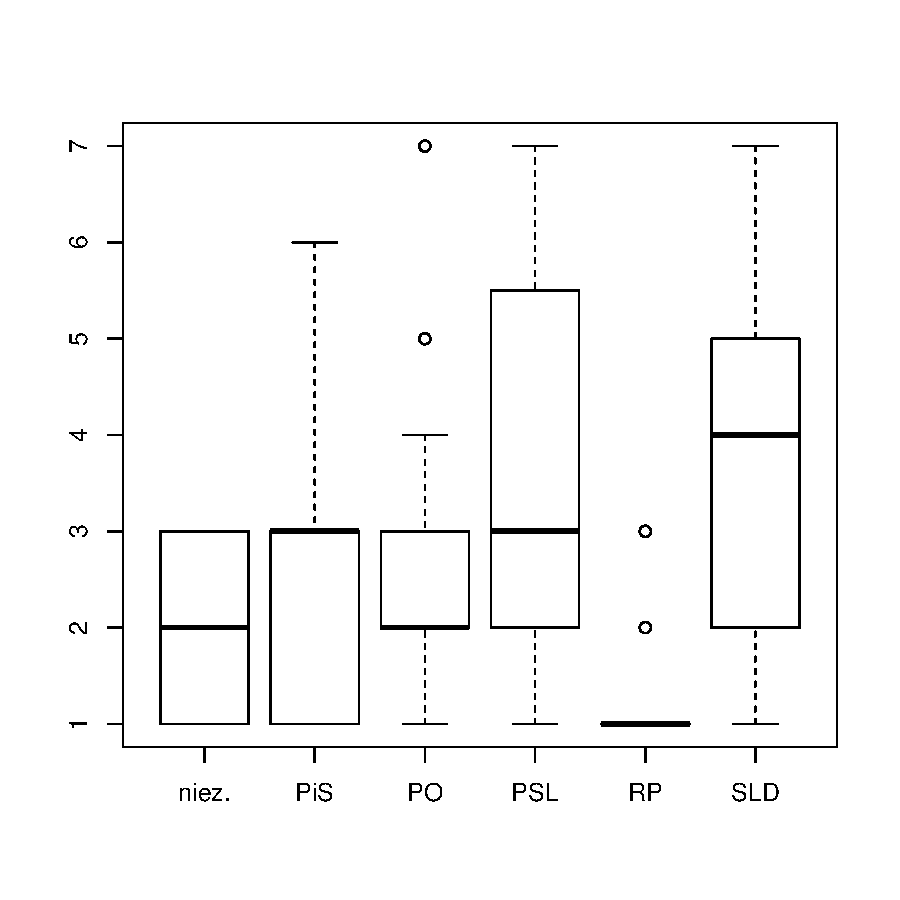
\includegraphics{sejm7_wg_stazu-002}
\caption{Średni staż posłów (wykres pudełkowy)}
\end{figure}

Średni staż posłów w~poszczegółnych klubach:

\begin{Schunk}
\begin{Sinput}
> tapply (poslowie$kadencje, poslowie$klub, mean)
\end{Sinput}
\begin{Soutput}
   niez.      PiS       PO      PSL       RP      SLD 
2.000000 2.352564 2.256039 3.535714 1.073171 3.576923 
\end{Soutput}
\end{Schunk}

Posłowie~7 kadencji Sejmu według klubów i~liczby kadencji:

\begin{Schunk}
\begin{Sinput}
> # http://ww2.coastal.edu/kingw/statistics/R-tutorials/descriptive.html
> table(poslowie$klub, poslowie$kadencje)
\end{Sinput}
\begin{Soutput}
         1  2  3  4  5  6  7
  niez.  1  0  1  0  0  0  0
  PiS   45 30 66 12  2  1  0
  PO    50 83 49 23  1  0  1
  PSL    5  6  6  1  3  4  3
  RP    39  1  1  0  0  0  0
  SLD    5  3  4  5  6  1  2
\end{Soutput}
\end{Schunk}

\end{document}
